In terms of comparing the decelerator concepts in terms of mass, the total decelerator mass as yielded by the methods outlined in section \ref{sec:strucmeth} is computed for each of the five concepts. Due to the limited applicability of each of the methods used, a necessity is the use of multiple methods: the method by Samareh \cite{Samareh2011} for the mass estimation of stacked toroid, tension cone and trailing \gls{iad} concepts; the method by Anderson \cite{Anderson1969} for the mass estimation of the isotensoid and the reference method for the mass estimation of the rigid concept. 

\begin{figure}[H]
\centering
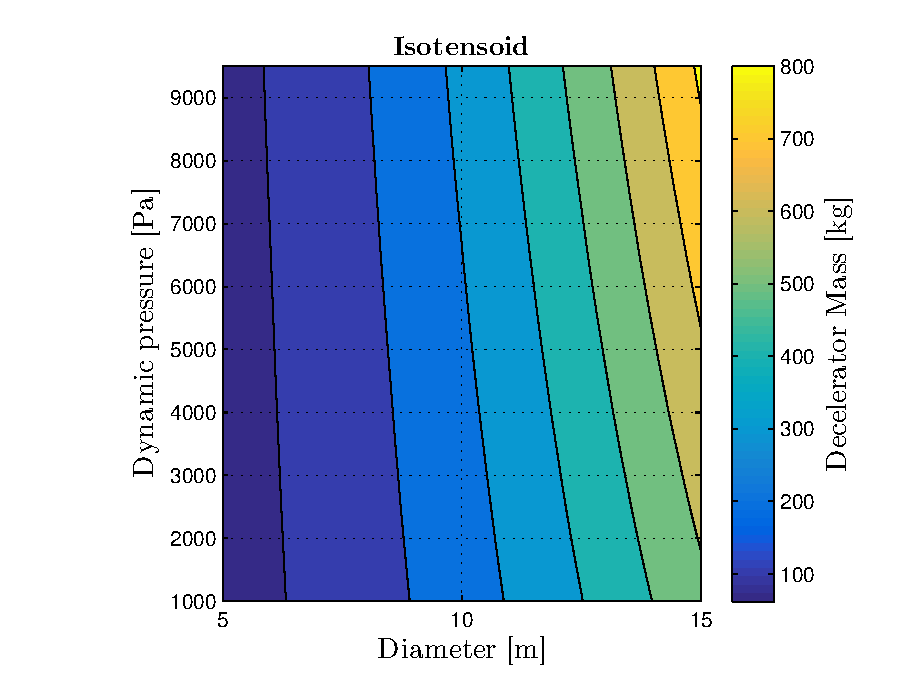
\includegraphics[width = 1.0\textwidth]{Figure/ISO_comp.eps}
\caption{\acrlong{dot} for mission duration}
\label{fig:ISO_comp}
\end{figure}





Figure \ref{fig:mass_dia} display the performance of all the inflatable concepts in one figure for a set value shape parameters. Figure \ref{fig:mass_dia} was made with a peak dynamic pressure of $\gls{sym:q}=3000$ [$Pa$], a drag coefficient $\gls{sym:CD}=1.5$ [$-$]. The Vectron material was used for.  .... en nu weet ik  niet wat jij hebt ingevuld...

Figure \ref{fig:mass_dia} serves to show how each different configurations mass scales with varying deployed diameter. It can be noted that the isotensoid configuration has a relatively, compared to the other inflatable concepts, high mass at the base diameter of five meters. This can be attributed to the fact that the isotensoid configuration features no deployed diameter. Different from the other inflatable concepts described by the model of Samareh in which the undeployed diameter has direct links the the mass of for example the gas system. The isotensoid configuration, among featuring no pressurised gas inflation system but rather ram-air, has no such diameter defined. The isotensoid is a single all compassing inflatable covering the whole payload. 

Although plotted for set values of the drag coefficient, peak dynamic pressure and further configuration parameters important remarks with respect to the isotensoid design can already be made. If looking solely of the structural mass performance of the decelerator concepts a isotensoid configuration is the least preferable. This is further reinforced by the sensitivity analysis of section \ref{sec:strucsens} in which configuration sensitivity is further considered. 

\begin{figure}[H]
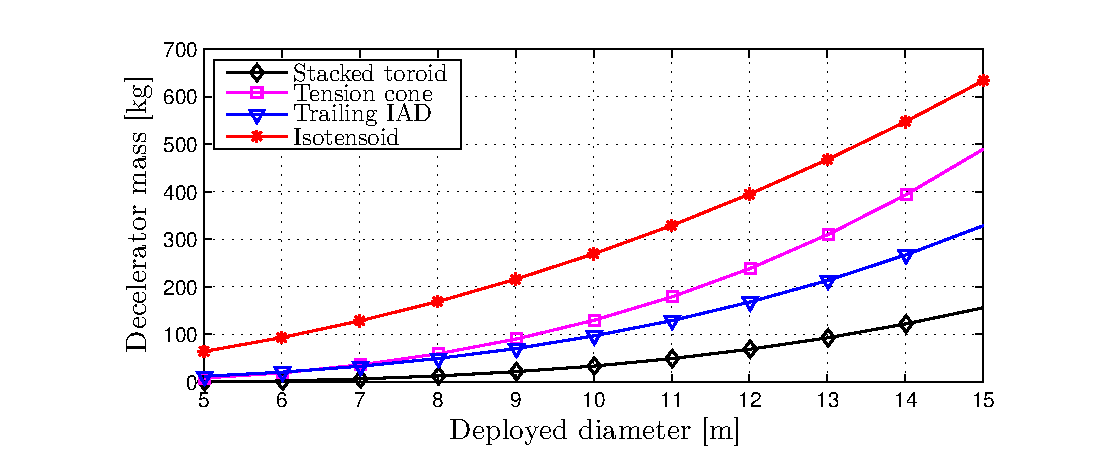
\includegraphics[width = 1.0\textwidth]{Figure/mass_dia.eps}
\caption{Decelerator mass versus deployed diameter for all the inflatable configurations}
\label{fig:mass_dia}
\end{figure}
